\expandafter\ifx\csname ifdraft\endcsname\relax
 \begin{document}
\fi

\section{結果}

\subsection{実験時条件}

実験は各プロトコル別日に行った.実験時の条件を以下に示す.

\begin{table}[H]
  \begin{center}
  \caption{低強度プロトコル}
  \label{tb:light_experiment}
    \begin{tabular}{ll}
      実験日 & 2021/01/24 \\
      開始時刻 & 18:21:54 \\
      体重 & 55.0kg \\
      気温(平均) & 12.99℃ \\
      大気圧(平均) & 1021.76hPa \\
      飽和水蒸気圧(平均) & 14.97hPa \\
      STPD係数(平均) & 0.95
    \end{tabular}
  \end{center}
\end{table}

\begin{table}[H]
  \begin{center}
  \caption{高強度プロトコル}
  \label{tb:hard_experiment}
    \begin{tabular}{ll}
      実験日 & 2021/01/25 \\
      開始時刻 & 9mm \\
      体重 & 55.0kg \\
      気温(平均) & 18.92℃ \\
      大気圧(平均) & 1027.19 \\
      飽和水蒸気圧(平均) & 21.88hPa \\
      STPD係数(平均) & 0.93
    \end{tabular}
  \end{center}
\end{table}

\subsection{結果グラフ}

以下に実験結果のグラフを示す.凡例は各グラフの下部に示した.

\subsubsection{低強度プロトコルと高強度プロトコルにおけるVO2}

\begin{figure}[H]
  \begin{center}
    \label{fig:light_hard_vo2}
    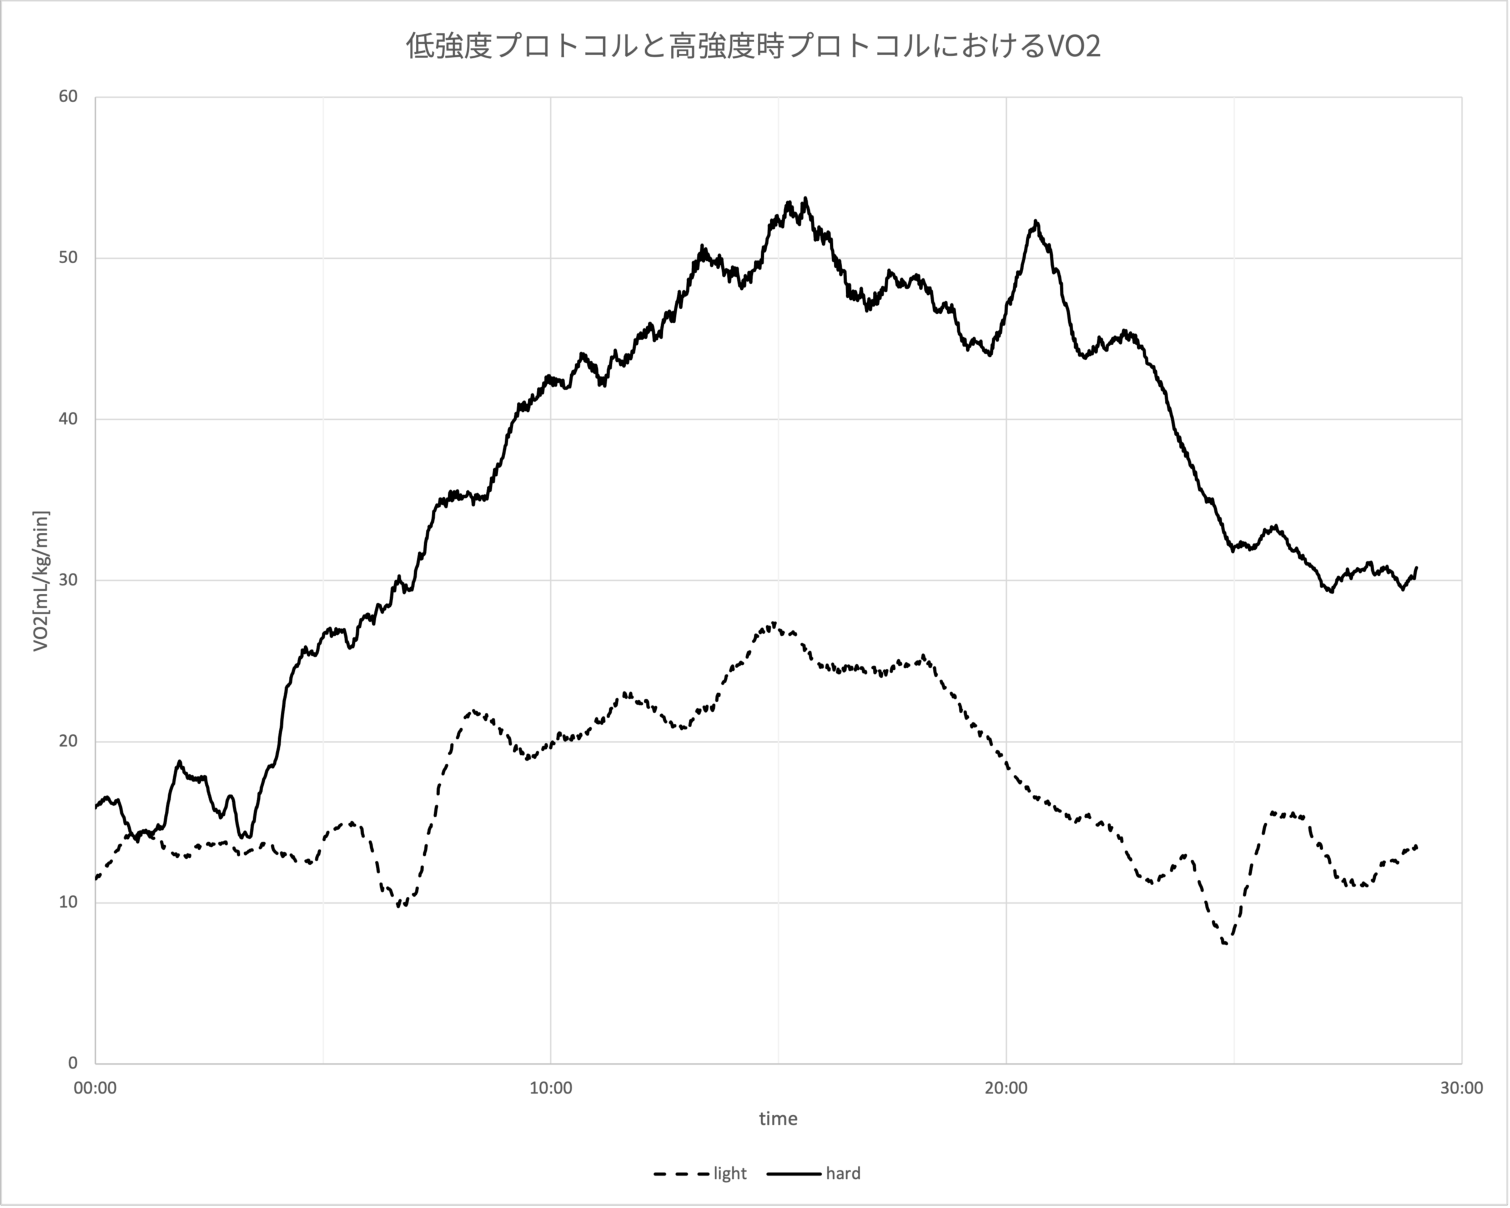
\includegraphics[width=12cm]{fig/light_hard_vo2}
    \caption{低強度プロトコルと高強度プロトコルにおけるVO2}
  \end{center}
\end{figure}

\subsubsection{低強度プロトコルにおけるVO2とパワー}

\begin{figure}[H]
  \begin{center}
    \label{fig:light_vo2_power}
    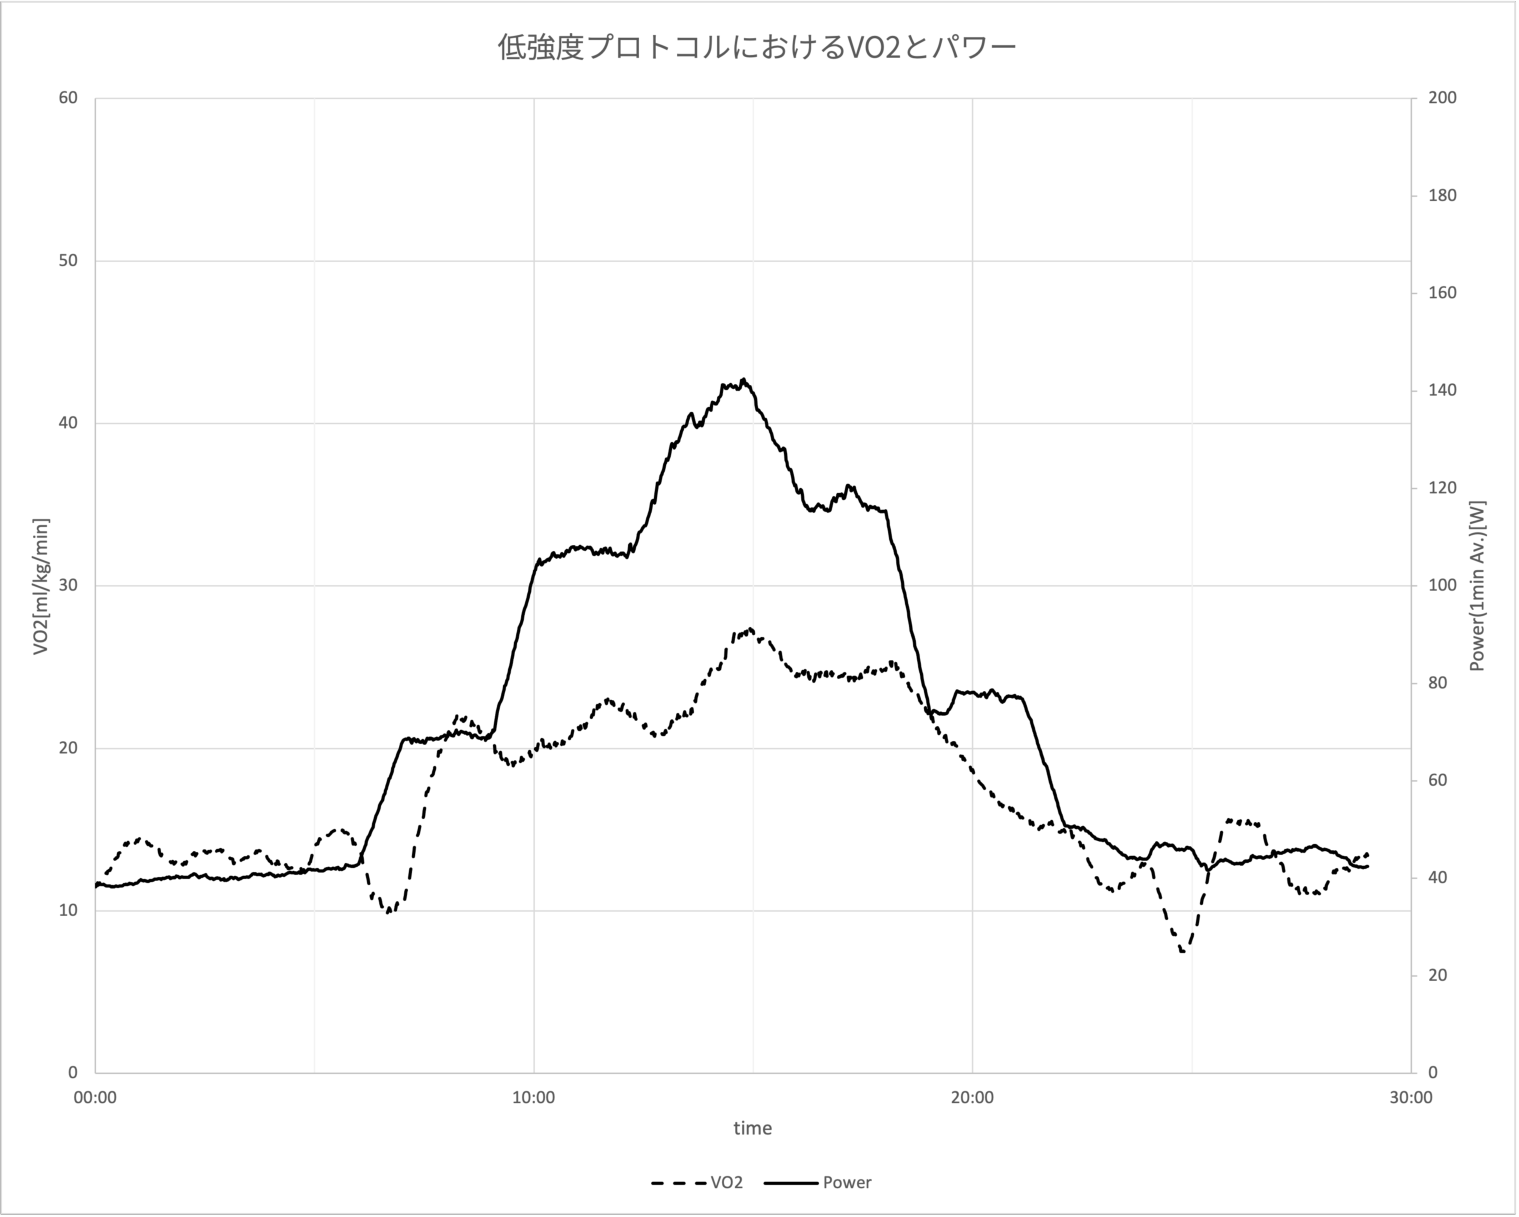
\includegraphics[width=12cm]{fig/light_vo2_power}
    \caption{低強度プロトコルにおけるVO2とパワー}
  \end{center}
\end{figure}

\subsubsection{低強度プロトコルにおけるVO2と心拍数}

\begin{figure}[H]
  \begin{center}
    \label{fig:light_vo2_hr}
    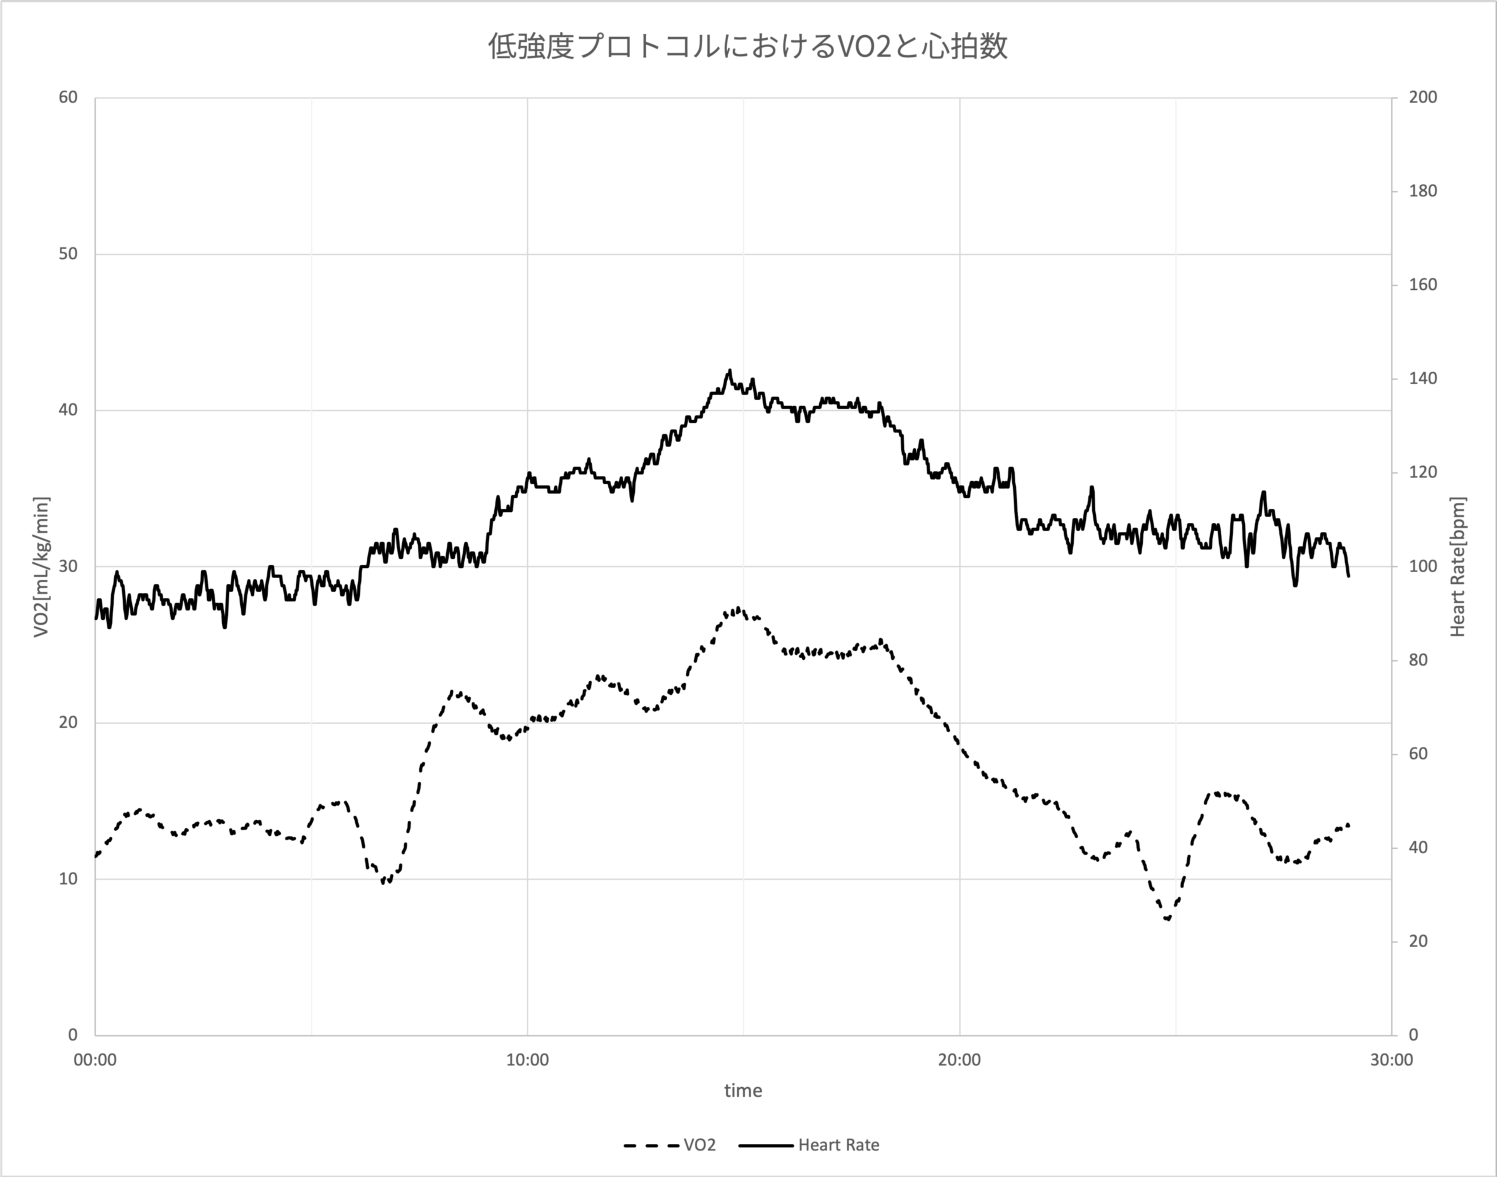
\includegraphics[width=12cm]{fig/light_vo2_hr}
    \caption{低強度プロトコルにおけるVO2と心拍数}
  \end{center}
\end{figure}

\subsubsection{高強度プロトコルにおけるVO2とパワー}

\begin{figure}[H]
  \begin{center}
    \label{fig:hard_vo2_power}
    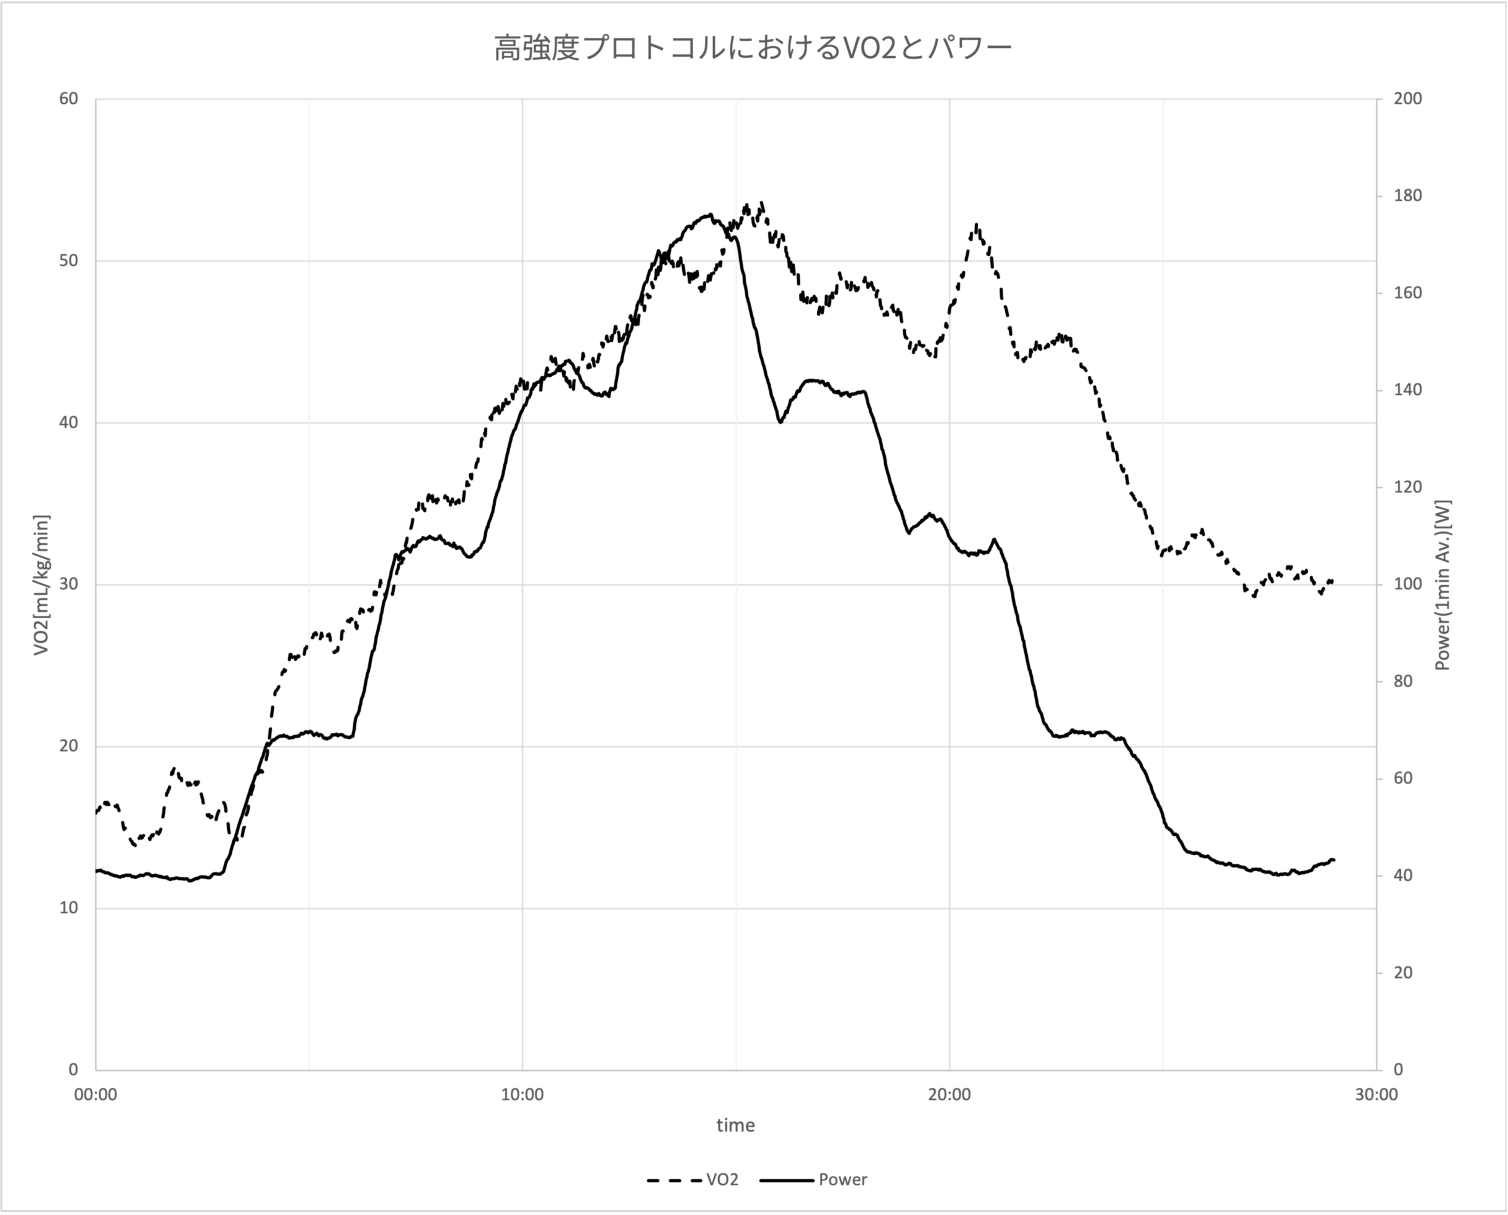
\includegraphics[width=12cm]{fig/hard_vo2_power}
    \caption{高強度プロトコルにおけるVO2とパワー}
  \end{center}
\end{figure}

\subsubsection{高強度プロトコルにおけるVO2と心拍数}

\begin{figure}[H]
  \begin{center}
    \label{fig:hard_vo2_hr}
    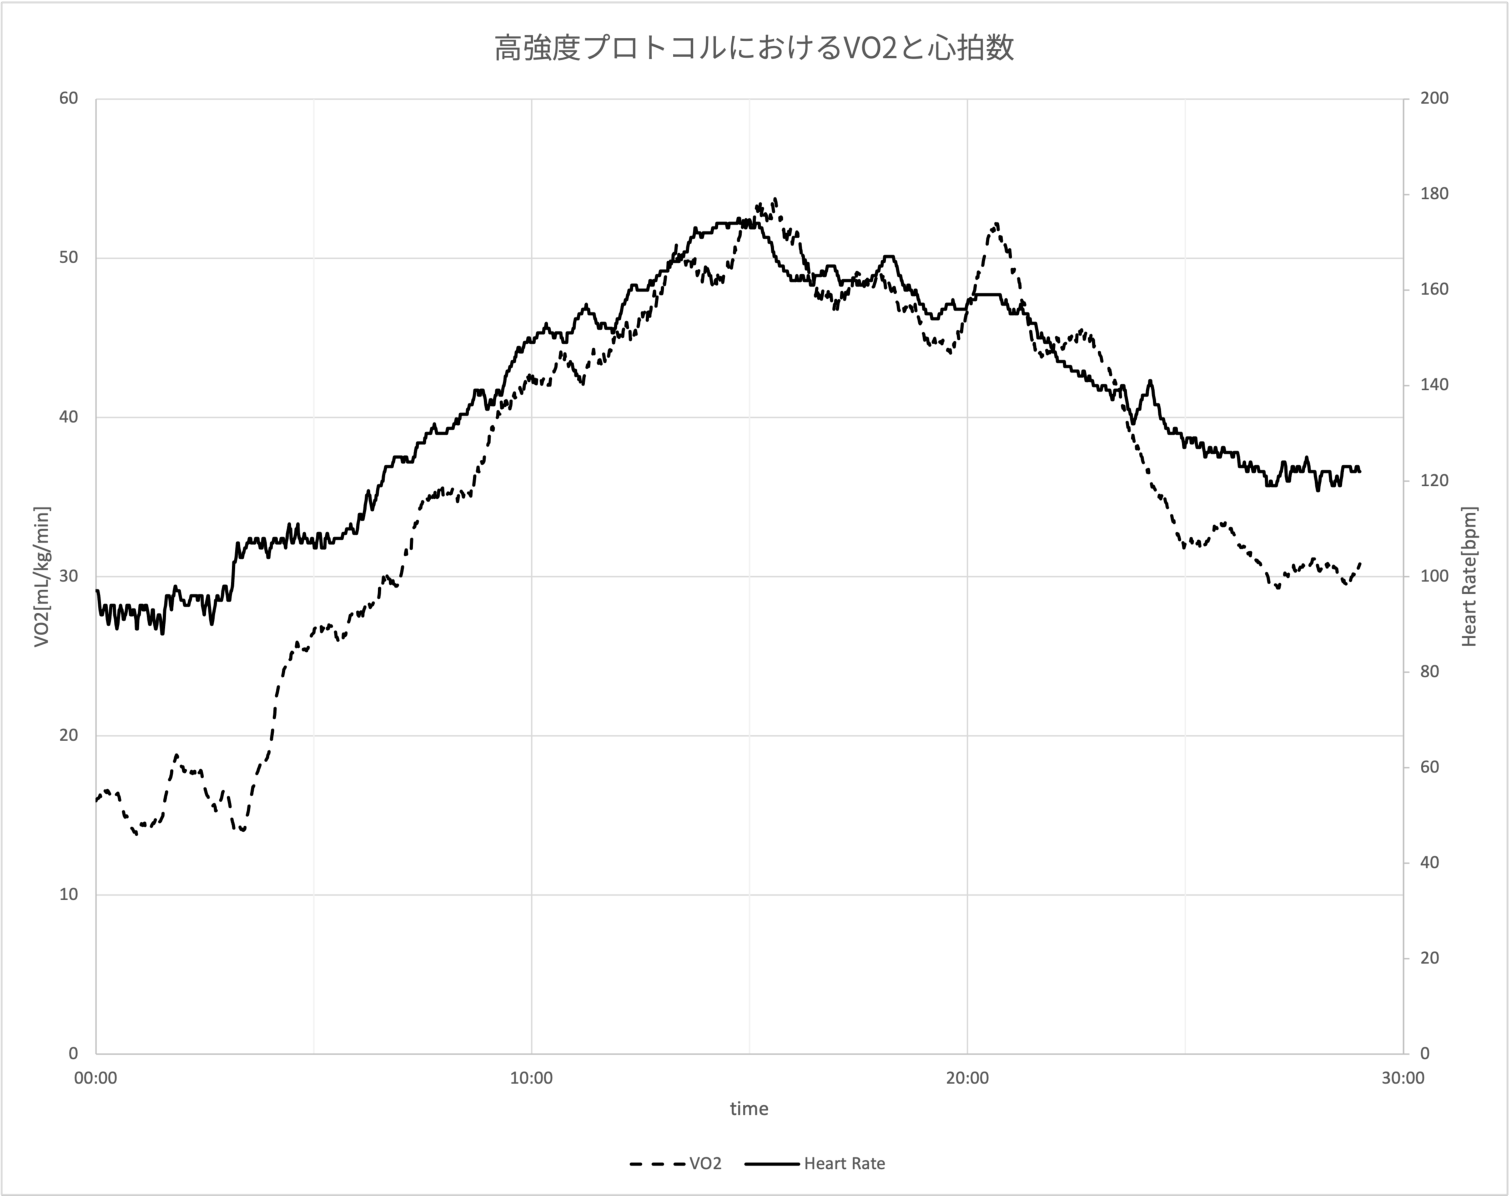
\includegraphics[width=12cm]{fig/hard_vo2_hr}
    \caption{高強度プロトコルにおけるVO2と心拍数}
  \end{center}
\end{figure}

\expandafter\ifx\csname ifdraft\endcsname\relax
  \end{document}
\fi
